\section{Direct-partial learning, representation, and readout}
\label{sec:direct_main}
This section supports the current main figures. It replaces their evidence
basis, not the identity of earlier records. Every displayed adaptive entry
is learned directly from observed incompatibility; none is produced by
fitting a physical residual coefficient and differentiating it. The current
code is in \path{experiments/direct_submission/}. Complete source snapshots,
configurations, observations, pre-update representations, and checksums
identify the executed versions.

\subsection{Common learning law and information boundary}
With fixed diagonal context units $D$, a local field is
$\widehat F=QD^{-1}$ and the observation is $v=D^{-1}\dot z_m$, or the
explicitly stated causal secant. At every sample, all entries of $Q$ are
free, with $QQ^{\mathsf T}=I$ and initially zero memory:
\begin{equation}
 \dot R=vv^{\mathsf T}-\lambda R,\qquad
 \dot Q=-\eta\{QR-(QRQ^{\mathsf T})Q\}.
 \label{eq:direct_common_law}
\end{equation}
For Fourier, substitute the lifted measured rate and its independent harmonic
field weights. This is the main paper's normalized law, not the sampled
physical-coefficient update in Section~\ref{sec:numerics}. The learner API
has observations, current representation/memory, units, and numerical settings;
it has no physical residual, true partial, simulator parameter, or oracle
coefficient initialization. No eigenvector replaces the adaptive update.

All observations over one numerical update are held. For forgetting time
$\tau=1/\lambda$, the memory used at each integration stage is
\begin{equation}
 R(s)=e^{-s/\tau}R_n+\tau(1-e^{-s/\tau})v_nv_n^{\mathsf T},
 \qquad 0\le s\le h_s.
 \label{eq:direct_stage_memory}
\end{equation}
Contact integrates the nonlinear normalized equation with DOP853 and a tiny
endpoint polar correction. The scalar Fourier row can equivalently normalize
the solution of $\dot a=-\eta R(s)a$: differentiating $a/\|a\|$ gives
(\ref{eq:direct_common_law}). This equivalence holds for evolving $R$.
Burgers uses subdivided RK4 with this same stage memory and unit retractions.
Independent joint-ODE comparisons test the actual numerical transitions.
Neither a frozen-memory exponential nor a batch eigensolver is mislabeled
as the evolving-memory law.

For a query, supply $v_S$ and compute
\begin{equation}
 \widehat v_C=-Q_C^\dagger Q_Sv_S.
 \label{eq:direct_common_readout}
\end{equation}
Units are restored before applying physical commands. When a command derivative
is returned, the command is integrated from its currently known value.
The main experiments do not reconstruct the physical simulator residual
for this operation. Conditioning guards and actuator restrictions remain
explicit. A guarded fallback, where present in the retained Burgers
challenge, is counted as a failure of learned completion, not a success.

\begin{table*}[t]
\centering
\caption{Information supplied to the current main learners and readouts.
Physical parameters and Jacobians are simulator/evaluator only in every row.}
\begin{tabular}{p{.12\textwidth}p{.31\textwidth}p{.25\textwidth}p{.225\textwidth}}
\toprule Study & Observations and supplied choices & Free learned entries & Readout and scope \\
\midrule
Fourier & Exact $x,\dot x$, noisy $\dot y$; known phase $20x$, order $K=1$, one constraint, units & Six independent harmonic weights; both evaluated entries free & Frozen learned field predicts a separate 30-s episode; one initial output calibration. \\
Contact & Ideal eight-channel context and its time rates; three constraints and declared units & All 24 entries of a local $3\times8$ row-orthonormal field & Same pre-update field completes acceleration/input rates for force and motion control; approximate subspace recovery. \\
Burgers & Ideal $w,w_t$, spatial derivatives of observed $w$, known $u$; causal $.05$-s context secants & Five independent entries at each of 32 sites; no supplied $w_t$ or input coefficient & Same pre-update rows return input rates; full sensing/actuation; separate causal/noisy challenges fail. \\
\bottomrule
\end{tabular}
\label{tab:direct_information}
\end{table*}

\subsection{Distinct interpretation of the diagnostics}
Pre-update energy measures compatibility with the actual measured/estimated
rate. Physical recovery uses $\|P_Q-P_{FD}\|_F$ in fixed units; a display gauge
is an evaluator operation and never changes the learner or command.
Readout error compares a learned completion with the physical completion of
the same supplied query, while task error compares the executed trajectory
with its reference. These are different quantities. A small task error need
not identify every direction, and a positive noisy covariance gap need not
identify the physical field. Physical-row energy on noisy or finite-secant
observations is a reference, not a universal minimum.

The learned local rows describe the visited trajectory. No globally
integrable residual or off-trajectory identification is inferred from the
plots. Main theorem statements and complete proofs remain in the main paper;
these numerical tests do not certify all their hypotheses. In particular,
contact's residual subspace error and small canonical material entry limit
physical coefficient interpretation, and Burgers' ideal sensing cannot be
replaced by an inaccurate derivative estimator without changing the outcome.

\subsection{Direct Fourier learning on a monotone graph}
\label{sec:direct_fourier_protocol}
This is the new protocol \path{direct_fourier_monotone_20261120_v1},
which supplies the current main Fourier learning and prediction evidence.
It is a nonlinear kinematic graph benchmark, not the earlier periodic dynamic
plant of Section~\ref{sec:normalized_fourier_results}. Its simulator uses
\begin{equation}
 y=.3+1.2x+.02\sin(20x),\qquad z=(x,y).
 \label{eq:df_graph}
\end{equation}
The formula and its physical row $F=(-1.2-.4\cos(20x),1)$ are used only by
the simulator and evaluator. The learner is given neither the residual
formula nor any physical coefficient, partial entry, or derivative target.
Both context units are fixed and dimensionless. It receives exact $x$ and
$\dot x$, noisy $\dot y_m=\dot y+\varepsilon_n$ with independent
$\varepsilon_n\sim\mathcal N(0,.0005^2)$, and known coordinate phase
$\phi=20x$. The phase and harmonic order $K=1$ are supplied representation
assumptions. Phase is derived from measured $x$, not an independently
manipulated physical input or an extra coordinate of $z$.

\paragraph{All-entry representation and coupled update.}
With $h=(1,\cos\phi,\sin\phi)^{\mathsf T}$, the unit row
$C\in\mathbb R^{1\times6}$ represents
\begin{align}
 \widehat H_C(x)&=C(h\otimes I_2),&
 w&=h\otimes(\dot x,\dot y_m)^{\mathsf T},\label{eq:df_lift}\\
 \dot R&=ww^{\mathsf T}-R/30,&
 \dot C&=-100\{CR-(CRC^{\mathsf T})C\}.
 \label{eq:df_update}
\end{align}
Every one of the six harmonic weights is independently adaptive, including
all three weights of the output entry. No potential is fitted and then
differentiated. Six independent standard-normal draws are normalized to
initialize $C$, without rejection or physical information; $R(0)=0$.
The initial $x_0$ is then drawn uniformly over one phase cycle. Seeds 10--19
vary these initializations and the sensor noise. The same-stream $K=0$
comparison learns a direct two-entry row from the identical measured
velocities, with the same gain, memory, and sample interval; its initial row
is the normalized first two entries of the $K=1$ initialization. This is an
ablation of the harmonic representation under matched settings, not a
comparison with an independently optimized alternative estimator.

Sampling is $\Delta t=.02$~s. Each observed $w_n$ is scored with the pre-update
row. Over its subsequent held-sample interval, the covariance is evaluated as
\begin{equation}
 R(s)=e^{-s/30}R_n+30(1-e^{-s/30})w_nw_n^{\mathsf T}.
 \label{eq:df_memory}
\end{equation}
DOP853 integrates $\dot a=-100R(s)a$, starting at $a(0)=C_n^{\mathsf T}$,
with relative and absolute tolerances $10^{-9}$ and $10^{-11}$; the returned
row is $a^{\mathsf T}/\|a\|$. Thus memory evolves within each integration
step. This implements the coupled normalized law, not a frozen-memory
exponential or an instantaneous bottom-eigenvector update. All coefficient
and covariance states before each observation are saved.

Training imposes coefficient normalization only; no all-phase row-norm
constraint is enforced. This is the unguarded normalized flow, not a feasible
projection onto the main paper's phase-constrained set. A postprocessing check
of saved states makes the distinction concrete: for seed 11 at $t=5.06$ s,
the learned field has norm $5.37\times10^{-5}$ at phase $-.675677$.
Thus a $.05$ all-phase row-norm bound would fail at that training state.
No prediction task uses these intermediate fields. Readout feasibility is
checked separately for the final frozen field below; the diagnostic and its
saved-state identity are retained in \path{row_norm_guard_diagnostic.json}.


\paragraph{Actual input and partial timescales.}
The training input over $0\le t\le240$~s is
\begin{equation}
 x=x_0+.15t+.05\sin(.3t),\qquad
 \dot x=.15+.015\cos(.3t).
 \label{eq:df_train_input}
\end{equation}
The actual supplied coordinate is a monotone ramp plus slow modulation;
its actual rate modulates at $.3$~rad/s. Physical partial variation follows
$\dot\phi=20\dot x\in[2.7,3.3]$~rad/s, nine to eleven times that modulation.
This comparison uses the executed input, not merely a desired reference.
The output rate $\dot y$ is fast and is not called a slow input.
For seed~10, the empirical derivative-RMS/centered-RMS rate scales are
$.01447$ for $x$, $.30100$ for $\dot x$, $3.00995$ for the physical slope,
and $2.91343$ for $\dot y$, in inverse seconds. The statistic for the ramp
$x$ depends on the observation duration and is not a stationary spectral
frequency. These diagnostics do not claim that every learner channel is slow.

\paragraph{Independent prediction using the same learned field.}
At 240~s learning stops. A new 30-s episode uses
\begin{align}
 x(t)&=x_{\rm final}+.12t+\frac{.03}{.47}(1-\cos(.47t)),\\
 \dot x(t)&=.12+.03\sin(.47t),\qquad 0\le t\le30~\mathrm{s}.
 \label{eq:df_test_input}
\end{align}
Its actual rate modulation is $.47$~rad/s, while the physical partial phase
rate lies in $[1.8,3.0]$~rad/s. With $C$ frozen, the original learned field
computes
\begin{equation}
 \widehat{\dot y}=-\widehat H_x\dot x/\widehat H_y.
 \label{eq:df_readout}
\end{equation}
The predicted output is integrated by the trapezoidal rule from one measured,
exact initial $y$. No later $y$ or $\dot y$ is supplied to the readout or
assimilated into the prediction. Supplied $x$ follows the prescribed actuator
motion, so it is not a hidden future output. Each seed learns on one
continuous training trajectory; the subsequent episode tests prediction and
is not an additional perturbation trial used for identification.

A query with $|\widehat H_y|<.05$ is invalid, with no oracle fallback.
Writing the output weights as $(C_{01},C_{11},C_{21})$ gives the elementary
all-phase bound
\begin{equation}
 |\widehat H_y|\ge |C_{01}|-\sqrt{C_{11}^2+C_{21}^2}.
 \label{eq:df_guard}
\end{equation}
The minimum final bound across all ten seeds is $.6195546$, and all 15,010
learned heldout queries pass the guard. This is a final frozen-model bound,
not a continuous-time guarantee during training: 376 recorded training
snapshots would fail the query guard, when no prediction task was requested.
The frozen initial $K=1$ prior has 916 invalid heldout queries in seven runs;
its full-episode errors are recorded as undefined in those cases, not
replaced by selected valid-query averages. The $K=0$ heldout queries have
no guard failures.

\paragraph{Separate learning, recovery, and task evidence.}
The physical row is evaluator-only. At each observed context, the record
contains $\tfrac12(\widehat H_C\dot z_m)^2$, the Frobenius difference between
the estimated and physical row projectors, and the separately scored task
errors. Row normalization/sign alignment is used only for display and never
changes the field used for a query. On $[200,240)$~s, the ten-seed mean
row-projector error is $(6.3912\pm1.3368)10^{-5}$, versus
$.150378\pm.000704$ for $K=0$. Mean observed pre-update energy is
$(4.8266\pm.1652)10^{-8}$, versus
$(3.66434\pm.01684)10^{-4}$ for $K=0$.
Prediction rate RMSE is $(1.60965\pm.46632)10^{-5}$ and integrated-output
RMSE is $(9.24323\pm6.70758)10^{-5}$. Corresponding $K=0$ errors are
$.0354751\pm.0001978$ and $.100628\pm.015898$.
All $\pm$ values denote sample standard deviations across the ten specified
seeds. Table~\ref{tab:direct_fourier_all_seeds} preserves every seed.

\begin{table*}[t]
\centering
\caption{New direct Fourier benchmark, all prespecified seeds. Projector
error is the mean on $[200,240)$~s; rate and output RMSE use the independent
30-s episode. Scaled columns indicate their multipliers in the headings.
The last column counts invalid queries of the frozen initial $K=1$ prior;
the trained $K=1$ and $K=0$ predictors have none.}
\label{tab:direct_fourier_all_seeds}
\begin{tabular}{rrrrrrr}
\toprule
Seed & \shortstack{Projector\\($10^{-5}$)} & \shortstack{Rate RMSE\\($10^{-5}$)} & \shortstack{Output RMSE\\($10^{-5}$)}
& \shortstack{$K=0$\\rate RMSE} & \shortstack{$K=0$\\output RMSE} & \shortstack{Prior\\invalid}\\
\midrule
10 & 5.9683 & 1.7412 & 12.5246 & 0.035598 & 0.109743 & 0\\
11 & 4.7770 & 1.4933 & 6.6561 & 0.034956 & 0.062450 & 0\\
12 & 7.7329 & 1.4550 & 5.0253 & 0.035570 & 0.110815 & 126\\
13 & 7.0664 & 1.9766 & 18.0278 & 0.035479 & 0.112136 & 0\\
14 & 5.3648 & 2.0516 & 22.4932 & 0.035639 & 0.102372 & 60\\
15 & 6.8780 & 1.6651 & 2.7531 & 0.035492 & 0.099707 & 256\\
16 & 5.4824 & 0.9637 & 3.2382 & 0.035392 & 0.085399 & 133\\
17 & 7.6658 & 2.0401 & 3.5015 & 0.035477 & 0.112295 & 101\\
18 & 8.3966 & 2.0018 & 10.8025 & 0.035527 & 0.111805 & 159\\
19 & 4.5798 & 0.7081 & 7.4099 & 0.035622 & 0.099562 & 81\\

\bottomrule
\end{tabular}
\end{table*}

\begin{figure*}[t]
\centering
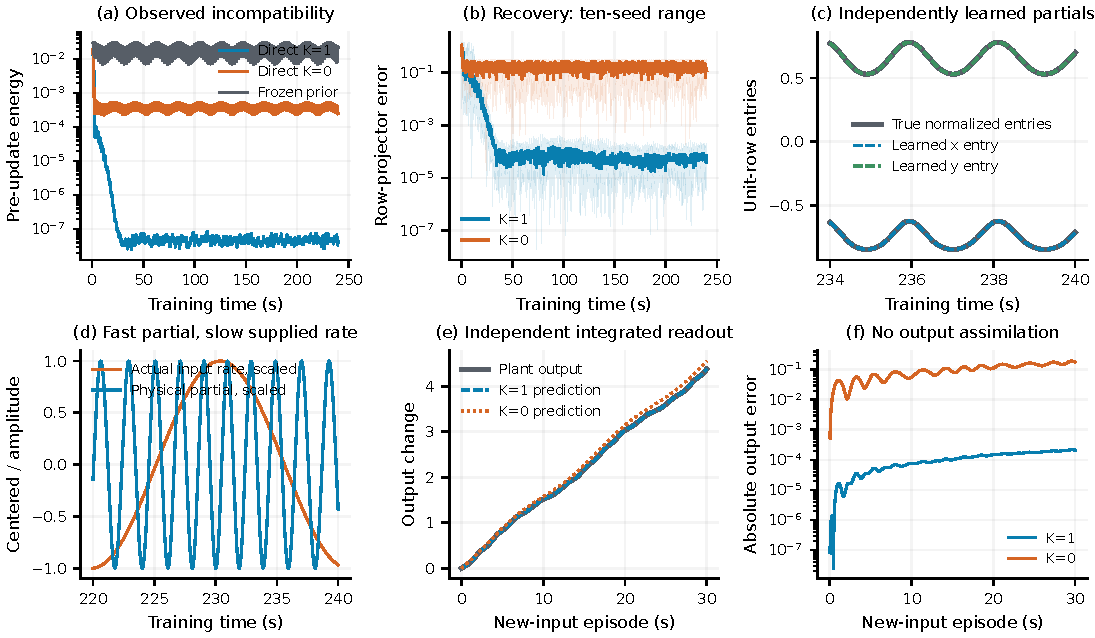
\includegraphics[width=.98\textwidth]{direct_fourier_summary.pdf}
\caption{Current direct Fourier evidence. Panels (a,c--f) use prospectively
selected seed~10; (b) shows the median and full range over all ten seeds.
Panel (a) is a causal 1-s mean of pre-update observed energy. Panel (c)
uses unit/sign alignment only for evaluating the two independently learned
entries. Panel (d) centers the actual input rate and physical partial and
divides each by its amplitude. Panels (e,f) integrate the same learned
readout on a new input, without later output assimilation.}
\label{fig:direct_fourier_new}
\end{figure*}

The final clean coefficient-covariance gap ranges from $.0054964$ to
$.0055467$, and $\|R_{\rm clean}C_*^{\mathsf T}\|$ is at most
$4.13\times10^{-15}$. Noisy covariance spectra and target-memory bias are
saved separately. A positive noisy eigengap is not treated as proof of
physical identification or unbiased recovery. All six coefficient entries
change in every run; the largest unit-norm error is $3.34\times10^{-16}$.
The generic learned field need not itself be a Jacobian. In this graph
geometry, wherever $\widehat H_y\ne0$, the gauge-equivalent field
$\widehat H/\widehat H_y=(\widehat H_x/\widehat H_y,1)$ is the gradient of
$y+\int (\widehat H_x/\widehat H_y)\,dx$. This post hoc interpretation does
not supply a potential to training and does not establish general
high-dimensional integrability.

\paragraph{Prespecification, verification, and provenance.}
The protocol fixed seeds 10--19, illustration seed~10, durations, observations,
initialization, baselines, and criteria before any new run. The excluded
exploratory pilot uses seed~9001. Each confirmatory seed passes the declared
limits: late mean projector error below $.01$, heldout rate RMSE below
$.002$, output RMSE below $.02$, and no learned heldout guard failure. These
are numerical evidence thresholds, not theorem hypotheses or significance
tests. No heldout result was used for tuning, and no run was omitted.

Two predeclared noise-free seed-10 refinements use $\Delta t=.02$ and $.01$~s.
Their final coefficient rows differ by at most $1.15\times10^{-14}$;
rate errors are below $1.84\times10^{-15}$ and integrated-output RMSE decreases
from $4.37321\times10^{-6}$ to $1.09337\times10^{-6}$. Direct projector
subtraction gives late errors below $10^{-14}$. The original equivalent
$\sqrt{2(1-\cos^2\theta)}$ summaries suffer cancellation at this scale and
report about $4\times10^{-9}$; those immutable summaries and the diagnosed
discrepancy are retained. This arithmetic floor is not interpreted as a
physical recovery error. The clean check isolates quadrature and update
accuracy, not a robustness test for noisy derivative estimation.

An independent audit reconstructs every recorded covariance transition,
observation/RNG stream, heldout rate and integrated trajectory. Selected
updates are checked against a tighter direct integration of the full
nonlinear coupled $(C,R)$ equations. All thirteen cases---the ten
confirmatory seeds, pilot, and two refinements---pass. The evaluator slope
is separately checked by finite differences of the simulator graph.
The portable source and commands are under
\path{experiments/direct_submission/fourier/}: \path{run.py},
\path{protocol.json}, \path{audit.py}, \path{summarize_plot.py}, and
\path{REPRODUCE.txt}. Each raw run retains source, configuration, complete
observed rates and pre-update coefficient/covariance states, predictions,
evaluator-only channels, RNG states, environment, and SHA-256 manifest.
The raw evidence archive is identified separately by the accompanying package manifest;
a local package does not imply that it has already been published.
The benchmark supports direct field learning and independent prediction
under known phase/order and the stated sensors. It does not validate the
old periodic plant's control, unknown-frequency discovery, noisy-rate
estimation from position-only sensors, or global stability.

\subsection{Direct local-field contact: protocol, readout, and limitations}
\label{sec:direct_contact_protocol}
The task is to regulate horizontal position $x$ and the vertical force
component $\lambda$ through a material/actuator change. The learner adapts all
$24$ entries of a local $3\times8$ field; its learned relations determine the
input-rate commands. This direct-field study is distinct from the retained
coefficient-family reconstruction and its geometry-dependent normal-force task.

\paragraph{Physical relation and observations}
The simulator uses $\dot p=Bu$, $p=(x,y)^{\mathsf T}$, and
\begin{align}
 \dot\lambda&=a\{h(x)-y\}-4\lambda+b\{h'(x)\dot x-\dot y\},\nonumber\\
 h(x)&=.035\sin2x+.020\cos5x.
 \label{eq:direct_contact_plant}
\end{align}
Initially $(a,b)=(600,240)$ and
$B=\left[\begin{smallmatrix}1&.15\\-.08&.85\end{smallmatrix}\right]$.
At $60$ s they change to $(1000,360)$ and
$B=\left[\begin{smallmatrix}.8&.22\\-.12&.65\end{smallmatrix}\right]$
without informing the learner. The initial state is
$(x,y,\lambda)=(0,.020-4/150,4)$.
The observed context and fixed units are
\begin{align}
 z&=(x,y,\lambda,v_x,v_y,r,u_1,u_2),\quad r=\dot\lambda,\nonumber\\
 D&=\operatorname{diag}(.3,.03,5,.15,.03,5,.15,.03),\quad
 v=D^{-1}\dot z.\label{eq:direct_contact_units}
\end{align}
On each smooth material branch, the plant obeys the three implicit relations
\begin{equation}
 f(z)=\begin{bmatrix}
 r-a\{h(x)-y\}+4\lambda-b\{h'(x)v_x-v_y\}\\
 v_x-B_{11}u_1-B_{12}u_2\\
 v_y-B_{21}u_1-B_{22}u_2
 \end{bmatrix}=0.
 \label{eq:direct_contact_relation}
\end{equation}
Writing $\gamma=a h'(x)+b h''(x)v_x$, the true field $F=D_zf$ is
\begin{equation}
 F=\begin{bmatrix}
 -\gamma&a&4&-b h'(x)&b&1&0&0\\
 0&0&0&1&0&0&-B_{11}&-B_{12}\\
 0&0&0&0&1&0&-B_{21}&-B_{22}
 \end{bmatrix}.
 \label{eq:direct_contact_true_field}
\end{equation}
Thus $F\dot z=0$ relates motion, force variation and actuation. These formulas
are simulator/evaluator-only: neither $f,F$ nor $a,b,B,h$ enters the learner or
controller. Supplied choices are context, units, three-constraint dimension,
initialization, learning settings and task references. A noise-free ideal
sensor supplies $z$ and its physical rate, including force rate and force
acceleration, from forward physics; no differentiation of noisy force data
is tested.

Commands are piecewise linear. At a sample, the observed rate is the left-hand
rate produced by the preceding command slope; the newly computed slope acts
over the next interval. At the material/actuator change, the sensor reports
the new branch's finite one-sided rates. The jump impulse of a discontinuous
context component is not assimilated as an ordinary derivative sample.
This is a piecewise-smooth simulation, not an impact or impulse-observation
model. The state is advanced by RK4 with the interval's appropriate material
branch and linearly varying command.

\paragraph{Direct learning from measured rates}
For seed $s$, a QR factorization of a generic $8\times3$ Gaussian matrix with
RNG seed $s+10000$ gives $Q_0$; $R_0=0$. The learned physical field is
$\widehat F=QD^{-1}$, with incompatibility $Qv=\widehat F\dot z$.
No entry is fixed to zero, one, or a prescribed sign, and no sparsity or
coefficient ties are imposed. The rows are normalized by the executed law:
\begin{align}
 \dot R&=vv^{\mathsf T}-.5R,\qquad QQ^{\mathsf T}=I_3,\nonumber\\
 \dot Q&=-100\{QR-(QRQ^{\mathsf T})Q\}.
 \label{eq:direct_contact_law}
\end{align}
At each $0.01$-s sample, the pre-update $Q$ forms the command and scores the
observed incompatibility. The current observed $v$ is then held during the
learning interval. Its covariance is integrated exactly as
$R(s)=e^{-.5s}R_n+2(1-e^{-.5s})v_nv_n^{\mathsf T}$, and DOP853 integrates
$Q$ against this evolving covariance, with relative/absolute tolerances
$10^{-10}/10^{-12}$. An endpoint polar correction removes numerical drift;
a raw orthogonality error greater than $10^{-7}$ aborts the run. An
instantaneous eigensolver is not substituted for the learning dynamics.
The evaluator obtains physical partials only after command construction.
Learning remains active for all $120$ s; at $40$ s, open-loop probing gives
way to feedback control.

\paragraph{Comparing learned and true partial relations}
Row-space agreement is measured in the fixed units by
$e_P=\|Q^{\mathsf T}Q-T^{\mathsf T}T\|_F$, where
$T=\{(FD)(FD)^{\mathsf T}\}^{-1/2}FD$ is the orthonormal true row frame.
For entrywise comparison, if $TQ^{\mathsf T}=U\Sigma V^{\mathsf T}$,
compare $OQ$ with $T$, where $O=UV^{\mathsf T}$ is evaluator-only.
This orthogonal alignment preserves column norms and row-space geometry,
not individual entry amplitudes. It does not enter learning or control;
the comparison concerns normalized partial relations, not unique canonical
values of $F$. For seed $101$ during control,
$\min\sigma(TQ^{\mathsf T})=.940553$; the orthogonal-factor error is below
$3.1\,10^{-15}$. The actual learned control block has minimum singular value
$.054216$, compared with $.127422$ for the orthonormal physical control block.
Small incompatibility is not reported as exact physical identification.

Canonical normalization fixes the $(r,u_1,u_2)$ columns $(6,7,8)$ by
inverting their unscaled learned block, whose minimum singular value reaches
$6.06\,10^{-6}$. This poorly conditioned inversion can produce inaccurate
material entries (Fig.~\ref{fig:direct_contact_canonical}). The controller
instead supplies $\dot r$ and solves the scaled $(v_y,u_1,u_2)$ block
$(5,7,8)$ for $(\dot v_y,\dot u_1,\dot u_2)$. Its regular completion can
therefore support useful regulation while the different canonical inversion
amplifies field errors. The evidence supports approximate local row-space
tracking, not precise material magnitudes, global integrability, or
unrestricted plant identification.
For seed $101$ in the primary window, the empirical bottom-three memory
subspace has mean projector distance $.28834$ from the physical row space,
while the learner--memory distance is $.09478$ and the third/fourth eigengap
is $.0003995$. These distinct diagnostics expose local-history bias and
tracking lag, rather than interpreting covariance positivity as physical
persistent excitation.

\begin{figure*}[p]
\centering
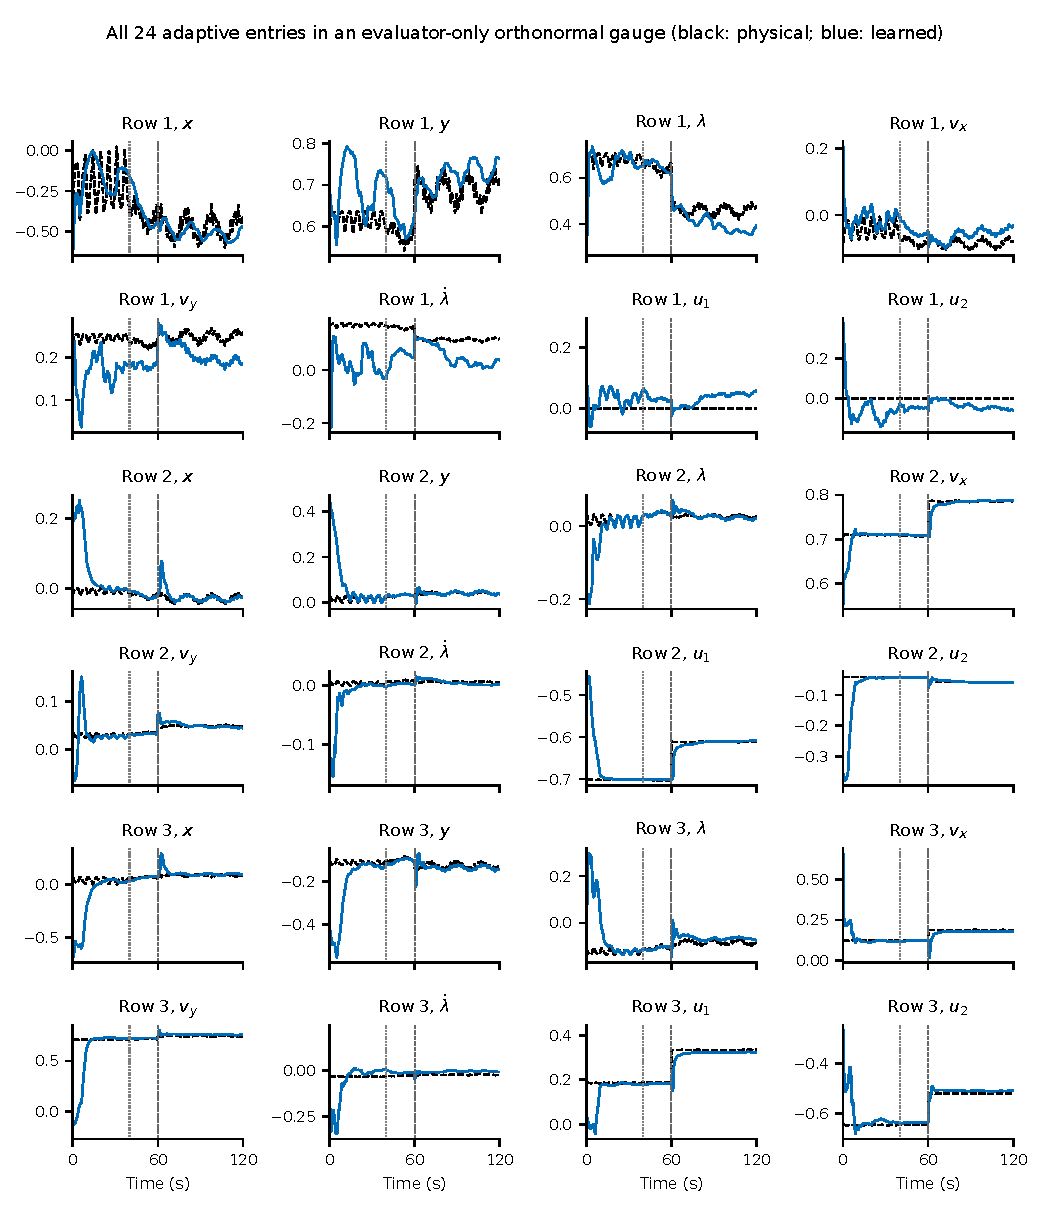
\includegraphics[width=\textwidth]{figures/direct_contact_all24.pdf}
\caption{Learning the contact relation: all $24$ adaptive entries for
preselected seed $101$. Each panel compares the same entry of the normalized
true field $T$ (black dashed) and aligned estimate $OQ$ (blue), using the
fixed units and evaluator-only orthogonal alignment defined in the text.
The learner receives no entries of $F$. Open-loop probing ends and control
begins at $40$ s (dotted line); learning continues throughout all $120$ s.
The material/actuator change occurs at $60$ s (dashed line).
Residual discrepancies remain visible; task success is not exact recovery
of every physical partial.}
\label{fig:direct_contact_all24}
\end{figure*}
\begin{figure}[t]
\centering
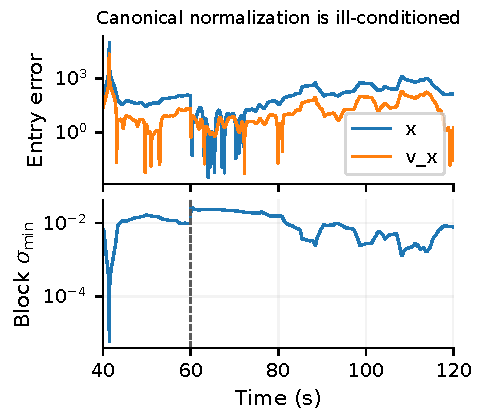
\includegraphics[width=\columnwidth]{figures/direct_contact_canonical_gauge_limitation.pdf}
\caption{A retained limitation: normalizing the material force-rate entry to
one is poorly conditioned and yields large physical-entry errors. This
normalization is evaluator-only and never used for commands or learning.}
\label{fig:direct_contact_canonical}
\end{figure}

\paragraph{Feedback and learned-field readout}
A measured open-loop warmup occupies $0\le t<40$ s:
\begin{align}
 u_1(t)&=.06\sin1.1t+.03\sin(2.3t+.4)\nonumber\\
       &\quad+.015\sin(3.7t+.2),\nonumber\\
 u_2(t)&=.002\sin(.9t+.8)+.0015\sin1.9t\nonumber\\
       &\quad+.001\sin(3.1t+.1).
 \label{eq:direct_contact_probe}
\end{align}
The applied warmup slope is the forward difference of these prescribed input
values across the next sample interval. This is an ordinary observed temporal
trajectory, not a source of independently labeled perturbation tangents.
After warmup, with $s=t-40$, the references are
\begin{align}
 x_d&=.03\sin(.35s)+.01\sin(2.3s)+.005\sin(3.7s),\nonumber\\
 \lambda_d&=4+.2\sin(.5s)+.08\sin(1.9s)+.04\sin(3.1s).
 \label{eq:direct_contact_reference}
\end{align}
Their derivatives are known task inputs; small independent components maintain
local excitation. Feedback prescribes $\dot v_x=a_x^*$ and
$\dot r=a_\lambda^*$:
\begin{align}
 a_x^*&=\ddot x_d-4(v_x-\dot x_d)-4(x-x_d),\nonumber\\
 a_\lambda^*&=\ddot\lambda_d-6(\dot\lambda-\dot\lambda_d)
                         -9(\lambda-\lambda_d).
 \label{eq:direct_contact_feedback}
\end{align}
The supplied rates are $(v_x,v_y,r,a_x^*,a_\lambda^*)$; the computed
rates are $(a_y,\dot u_1,\dot u_2)$. Using one-based columns
$S=(1,2,3,4,6)$ and $C=(5,7,8)$, the same pre-update relation
$\widehat F\dot z=0$ gives
\begin{equation}
 \begin{bmatrix}a_y\\\dot u_1\\\dot u_2\end{bmatrix}
 =-D_CQ_C^{-1}Q_SD_S^{-1}
 \begin{bmatrix}v_x\\v_y\\r\\a_x^*\\a_\lambda^*\end{bmatrix}.
 \label{eq:direct_contact_completion}
\end{equation}
Desired rates enter this query only; learning still uses observed $v$.
Only the last two completed components are applied: their limited slopes
update the measured input by $u_{n+1}=u_n+\Delta t\,\dot u_n$.
The inferred $a_y$ closes the relation but is not a separate actuator command.
Limits are $|u_i|\le.8$ and $|\dot u_i|\le5$.
If $\sigma_{\min}(Q_C)<.005$, the trajectory is recorded as failed and stops;
there is no physical inverse or fallback controller. Domain checks stop a run
if indentation or force is nonpositive, $|x|>1$, $|y|>.3$, or $|\lambda|>100$.
The prescribed control law contains neither $a,b,B$ nor $h$.

\paragraph{Task results and retained failures}
Exploratory seed $0$ was separate from confirmation. Its first, less excited
reference reached a readout guard at $58.58$ s and is retained as a failure.
The local references in~(\ref{eq:direct_contact_reference}) completed both a
60-s constant-plant pilot and a 120-s pilot with the scheduled change.
The learning gain, memory, units, and guard were unchanged. The measured
conditioning and task response motivated the reference revision; physical
partial errors were not feedback or selection inputs.

The complete protocol and source hashes were fixed before seeds
$101$--$105$, with seed $101$ preselected for illustrations. These seeds vary
generic field initialization; they are not five independently drawn plants or
noise realizations. The declared primary window was $[110,120)$ s. Criteria
required complete 120-s trajectories, no domain/guard/saturation event,
position RMSE below $.01$, vertical-force RMSE below $.2$, mean row-projector
error below $.6$, and field, incompatibility, and query errors below half their
respective frozen-initial same-stream values. All five runs met these
criteria; no seed was discarded.

\begin{table}[t]
\centering\small\setlength{\tabcolsep}{2.5pt}
\caption{All declared direct-contact runs, primary window $[110,120)$ s.
$e_P=\|Q^{\mathsf T}Q-P_{FD}\|_F$ in the fixed units of
(\ref{eq:direct_contact_units}). Query error is RMS norm over all three
completed physical rates. The frozen estimate is a same-stream shadow.}
\label{tab:direct_contact_seeds}
\begin{tabular}{rccccc}
\hline
Seed & Force RMSE & Position RMSE & Mean $e_P$ & Query RMS & Pass\\
\hline
101 & .121637 & $6.8111\,10^{-5}$ & .298169 & .00717262 & Yes\\
102 & .121637 & $6.8110\,10^{-5}$ & .298169 & .00717265 & Yes\\
103 & .121636 & $6.8112\,10^{-5}$ & .298169 & .00717260 & Yes\\
104 & .121642 & $6.8105\,10^{-5}$ & .298170 & .00717283 & Yes\\
105 & .121636 & $6.8113\,10^{-5}$ & .298169 & .00717260 & Yes\\
\hline
\end{tabular}
\end{table}
Across the five seeds, force RMSE is $.121638\pm2.31\,10^{-6}$,
position RMSE is $(6.81102\pm.00031)10^{-5}$, and mean projector error is
$.298169\pm6.15\,10^{-7}$ (sample standard deviations). The frozen projector
error is $1.93389\pm.16981$. Mean incompatibility norm is $.00359588$ versus
$.511730$ for frozen initialization. Query RMS is $.00717266\pm9.66\,10^{-8}$
versus $.214812\pm.100090$ for the frozen shadow. Query comparison supplies
the same requested rates to the learned and physical fields; it is an
inverse-readout diagnostic, not an independent future-prediction experiment.
Own-trajectory force/motion errors separately test the applied readout.

\paragraph{Numerical and provenance checks}
Saved records include every pre-update $Q,R,z,\dot z$, command, supplied query,
physical evaluator field, source snapshot, configuration, and per-file hash.
Recalculation from raw records reproduced trace metrics and controller outputs.
The covariance transition error is at most $1.12\,10^{-14}$; independent
200-substep RK4 checks of selected learning intervals agree within
$2.57\,10^{-12}$ in $Q$. Every entry changed, with the smallest across-entry
maximum change exceeding $.1185$ over the audited runs. Directional finite
differences check the evaluator partials separately from the learning rule.

The predeclared seed-$101$ refinement halves the observation/plant step to
$.005$ s, with all other settings unchanged. It also completes and passes the
criteria. Its force RMSE is $.109237$, versus $.121637$ at $.01$ s; projector
error is $.297450$, versus $.298169$. The same-time late force trajectories
differ by RMS $.01490$ N, and projector-error traces by RMS $.001719$.
Thus qualitative success is preserved, but fine quantitative force accuracy
is discretization-sensitive; the coarse records have not been replaced or
called a converged continuous-time solution.

The portable implementation, frozen protocol, auditing and plotting programs
are under \texttt{experiments/direct\_submission/contact/}. This new identity
has nine recorded executions: three exploratory cases, five confirmation
seeds, and one refinement. The earlier experiments using noisy measured
signals and cascaded causal differentiation are different protocols; their
failures remain archived and do not establish robustness for this study.
Local records and hashes are evidence of execution,
not a claim that a new archive or code revision has already been published.

\subsection{Direct five-entry Burgers learning and distributed readout}
\label{sec:direct_burgers_protocol}

This experiment replaces the prescribed three-coefficient Burgers learner in
its role as main-paper evidence. The earlier coefficient-family experiment
remains a separate historical protocol. Here every entry of a local differential
row is learned directly from observed context-rate incompatibility; the physical
Burgers coefficient family is used only to generate and evaluate the plant.
The protocol was fixed before running the five initializations and subsequent
sensor and timestep conditions. The main figure uses the preselected seed 732
and spatial site 0, without selection by the outcome.

\subsubsection{Plant, observations, and free differential row}
On the periodic domain $s\in[0,2\pi)$, the simulator is
\begin{equation}
 w_t+w w_s-.08w_{ss}-u=0,
 \qquad z=(w,w_s,w_{ss},u,w_t).
 \label{eq:direct_burgers_plant}
\end{equation}
A 32-point Fourier collocation grid and RK4 advance the physical state with
piecewise-linear $u$. All spatial points are sensed and actuated. The initial
state is $w(s,0)=.2+.015\sin s$, with $u(s,0)=0$. Fixed identity context scales
are used. At each site the learner stores an independent row
$q\in\mathbb R^{1\times5}$ and a $5\times5$ memory matrix. Every entry of $q$
is initialized from a generic Gaussian draw, followed by unit normalization.
The five initial seeds are 732--736; the independent sensor seed is the initial
seed plus 100000. No coefficient estimate, known partial entry, sparse physical
pattern, physical eigenspace, or true-$F$ initialization is supplied.

In the ideal condition, $w$ and $w_t$ are measured exactly; spatial channels
are spectral derivatives of the measured field. This is an explicit ideal
sensor assumption, not a noisy position-only result. The learner does not
receive an exact $w_{tt}$ sensor: its observation is the causal context secant
\begin{equation}
 v_k=\frac{z(t_k)-z(t_k-.05)}{.05},\qquad t_{k+1}-t_k=.005\,\mathrm{s}.
 \label{eq:direct_burgers_observation}
\end{equation}
After the first valid history window, it integrates
\begin{equation}
 \begin{aligned}
 \dot R&=v_kv_k^T-R/4,\\
 \dot q&=-10^4\{qR-(qRq^T)q\},\qquad qq^T=1.
 \end{aligned}
 \label{eq:direct_burgers_law}
\end{equation}
The secant is held during the current $.005$-s observation interval, but the
memory evolves throughout the representation update. Each RK4 stage evaluates
\begin{equation}
 R(t_k+\delta)=e^{-\delta/4}R_k+
               4(1-e^{-\delta/4})v_kv_k^T.
 \label{eq:direct_burgers_memory}
\end{equation}
At least four subdivisions are used; their length $d$ obeys
$10^4d\max\{\operatorname{tr}R_k,\operatorname{tr}R_{k+1}\}\leq.25$
across sites. Unit normalization follows each subdivision. This is numerical
integration of the coupled law, not replacement of learning by a bottom
eigenvector or descent with a frozen memory matrix.

\subsubsection{Training and same-field rate completion}
For $0\leq t<80$ s the input-rate probe is
\begin{equation}
 \begin{aligned}
 \dot u&=.01\sum_{k=0}^{3}\omega_k
       \sin((k+1)s+.37k)\cos(\omega_kt),\\
 &(\omega_0,\ldots,\omega_3)=(3,5,7,11).
 \end{aligned}
 \label{eq:direct_burgers_probe}
\end{equation}
Before observing $t=80$ s, the complete plant, input, learned row, memory,
observation histories and random-number state are cloned. One arm continues
learning and the other holds $q$ fixed. Both act on their own physical
trajectories until $t=100$ s. The fixed arm may evolve a diagnostic memory;
that memory does not update its row.

The target is
\begin{equation}
 w_d=.2+.015\sin s\cos(.3t)+.01\cos(2s)\sin(.5t).
 \label{eq:direct_burgers_reference}
\end{equation}
At each controlled sample, measured channels and the pre-update row form the
query before the current secant is assimilated. Set
\begin{equation}
 a_d=(w_d)_{tt}-4(w-w_d)-4(w_t-(w_d)_t).
\end{equation}
The supplied rates are $v_S=(w_t,(w_t)_s,(w_t)_{ss},a_d)$ and the computed
channel is $v_C=\dot u$. The same learned row returns
\begin{equation}
 \dot u=-\frac{q_w w_t+q_{w_s}(w_t)_s+q_{w_{ss}}(w_t)_{ss}+q_{w_t}a_d}{q_u}.
 \label{eq:direct_burgers_completion}
\end{equation}
A query with $|q_u|<.1$ uses the declared model-independent input decay $-u$
and is counted as guarded, not successful learned completion. Applied input
rates are clipped to $[-5,5]$; $\max_s|w|>5$ stops a branch. There is no
physical-model fallback. The ideal cohort has no guarded or clipped controlled
sample and no stopped branch; its smallest controlled $|q_u|$ is $.67137$.

\subsubsection{Separate recovery, compatibility, and task scores}
Only the evaluator forms the physical row
$F=(w_s,w,-.08,-1,1)$ at each branch's actual clean context. Let
$p=F/\|F\|$. The physical recovery metric is
\begin{equation}
 e_F=\|q^Tq-p^Tp\|_F=\sqrt{2(1-(qp^T)^2)}.
 \label{eq:direct_burgers_score}
\end{equation}
It is invariant to row sign and scale and ranges from zero to $\sqrt2$.
Entry plots use unit normalization and evaluator-only sign alignment; this
display convention never changes the learner or controller. Pre-update
incompatibility is scored separately as $\frac12(qv_k)^2$. Task RMS is the
root mean square of $w-w_d$ over all sites and applied observations in the
specified window. Terminal commands at $t=100$ are stored but not applied and
are excluded from task/readout metrics. Rendering uses every fifth sample;
metrics use every applied sample without smoothing.

\begin{figure}[t]
 \centering
 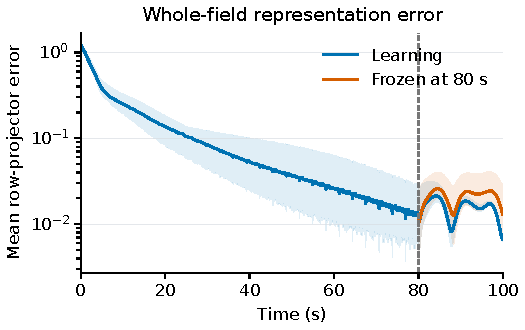
\includegraphics[width=\columnwidth]{figures/direct_burgers_diagnostics.pdf}
 \caption{Whole-field Burgers representation error, complementing the main
figure's partial, incompatibility and control plots. Curves are means and bands
span all five seeds, with error averaged over all 32 spatial sites. At 80 s,
the shared probing trajectory branches into separately controlled adaptive
and frozen runs. The adaptive rows continue learning through 100 s;
the frozen rows retain their values at 80 s.}
\label{fig:direct_burgers_protocol}
\end{figure}

\begin{table*}[t]
\centering
\caption{All ideal main-cohort outcomes. Late means/RMS use $[96,100)$ s.
The training qualification uses $[76,80)$ s and all the criteria stated in the text.
The final row gives the across-seed mean $\pm$ sample standard deviation.}
\label{tab:direct_burgers_ideal}
\renewcommand{\arraystretch}{1.15}
\begin{tabular}{c c c c c c}
\hline
Seed & Training qualified & Adaptive $e_F$ & Frozen $e_F$ &
Adaptive task RMS ($10^{-6}$) & Frozen task RMS ($10^{-6}$)\\
\hline
732 & No & .013761 & .018433 & 8.5084 & 22.4895\\
733 & No & .013222 & .021239 & 8.5186 & 25.8758\\
734 & Yes & .013231 & .014272 & 8.4460 & 11.7942\\
735 & No & .014729 & .037314 & 8.9005 & 49.9873\\
736 & Yes & .013344 & .015503 & 8.4874 & 13.9083\\
\hline
All five & 2/5 & $.013658\pm.000638$ & $.021352\pm.009323$ &
$8.5722\pm.1856$ & $24.8110\pm15.2371$\\
\hline
\end{tabular}
\end{table*}

The prospective training qualification requires mean $e_F\leq.05$, pooled
95th percentile $\leq.1$, maximum $\leq.25$, worst-site mean $\leq.1$, and
mean error at most one quarter of the initial-row same-stream error. Only
seeds 734 and 736 pass every condition. All five pass the inherited weaker
mean/reduction check and all five pass the declared adaptive late conditions:
mean $e_F\leq.1$, 95th percentile $\leq.25$, task RMS $\leq10^{-3}$,
guard and clipping fractions each strictly below $.01$, and completion to
100 s. These are offline labels, never training stops or feedback gates.
The five-seed result therefore demonstrates continued direct learning and
readout, not uniformly qualified tracking after convergence.

Over the full $[80,100)$ control interval, adaptive and frozen task RMS are
$.001223645\pm.000000231$ and $.001223943\pm.000000617$, respectively.
Their common initial transition dominates this interval; the late advantage
must not be described as a large full-horizon improvement. For the two
qualified seeds, frozen readout already works well and continued learning
provides a modest late improvement. The remaining seeds include continuing
recovery from incomplete training.

Even ideal sensing does not make the finite secant exactly tangent to the
instantaneous physical relation. The physical unit-row half-mean-square
secant energy is $4.4414\times10^{-11}$ over $[76,80)$ and averages
$1.5610\times10^{-13}$ on the adaptive late trajectories. The latter learned
energy is $3.6992\times10^{-10}$. Thus neither numerical zero compatibility
nor exact physical identification is claimed. The local time-varying rows
need not define an integrable global Jacobian field.

\subsubsection{Sensor failures and numerical refinement}
The complete study retains 19 cases: five ideal, five causal-clean and five
causal-noisy main cases, plus two ideal and two causal-clean refinements.
In causal cases a quadratic endpoint least-squares fit to the preceding $.10$
s of measured positions estimates $w_t$; the same estimate supplies both the
context and controller. No future samples or true-rate fill are used. Noisy
cases add independent position noise with standard deviation $10^{-5}$ per
site/sample. The causal secant first becomes valid at $.15$ s. Noise and row
initializations vary together across the five paired seeds; this is not a
crossed factorial noise study.

\begin{table}[t]
\centering
\caption{Main-cohort outcomes, retaining every seed. ``Late pass'' requires
all combined adaptive recovery, task, guard and completion criteria.}
\label{tab:direct_burgers_conditions}
\renewcommand{\arraystretch}{1.15}
\begin{tabular}{lccc}
\hline
Sensing & Training qualified & Late pass & Complete A/F\\
\hline
Ideal & 2/5 & 5/5 & 5/5, 5/5\\
Causal clean & 0/5 & 0/5 & 5/5, 0/5\\
Causal noisy & 0/5 & 0/5 & 5/5, 5/5\\
\hline
\end{tabular}
\end{table}

Every causal-clean frozen main branch reaches the declared field bound at
83.2 s. The two causal-clean frozen refinements stop at 83.2 and 83.2025 s.
Failed observations and unexecuted commands remain in the raw records; absent
late windows are not extrapolated. The causal-clean training discrepancy is
principally a biased observed covariance target: for seed 732 the learned,
observed-bottom and clean-bottom physical errors are $.479532$, $.480820$
and $.004098$, respectively. Small observed incompatibility does not identify
the physical partials. In the noisy cohort, adaptive late mean physical error
is $1.41362$, task RMS is $.007956$, and the guard fraction is one. Continued
adaptation under that sensor model is not successful partial recovery.

For preselected seed 732, the whole-loop step is halved from $.005$ to $.0025$
and $.00125$ s, keeping physical windows fixed. Ideal late mean field changes
are $2.11605\times10^{-5}$ and $9.60095\times10^{-6}$; the first exceeds the
prospective absolute $10^{-5}$ sensitivity flag, while neither exceeds the
10\% relative flag. Worst-site training means $.104301$, $.100618$ and
$.098807$ cross the qualification boundary only at the finest step. That
favorable result does not replace the prespecified main-cohort count of 2/5.
The second causal-clean halving changes late field error by 18.70\% and task
RMS by 38.39\%, so its whole-loop sensitivity test fails. Halving the loop
changes sensing, sampling and control as well as integration; it is not a
pure solver-order or continuous-PDE convergence test.

\subsubsection{Reproduction and audit boundary}
The portable package is
\path{experiments/direct_submission/burgers/}.
Its \path{protocol.json} preserves the original prospective declaration;
\path{source_mapping.json} distinguishes unchanged scientific functions from
local import, command-line and provenance adaptations. The package includes
compact full-sample plot trajectories, selected complete original chunks and
checkpoints, and all-condition summaries. These selected files are not the
complete 6.63-GB original raw archive, which remains a separate artifact;
no public download location is implied here.

The independent final-pass reconstruction checks the hashes of all 610 ideal
raw chunks and reproduces 200 metric comparisons. Every controlled command
is reconstructed from the saved pre-update row and observed supplied rates;
the largest discrepancy is $1.39\times10^{-17}$. Portable-source replay of
600 archived samples across training, adaptive and frozen phases is bitwise
identical. An independent literal joint-$q/R$ ODE check gives a row discrepancy
$1.51\times10^{-10}$, with successive held-observation halving errors
$9.29\times10^{-12}$ and $5.77\times10^{-13}$. The historical independent
audit also retains all 19 cases, sensor/filter reconstruction, coupled-ODE
checks and failed branch records.

From the package directory, \path{verify_package.py} performs the focused
replay/numerical checks, \path{plot_figure_focus.py} regenerates the current
figures without simulation, \path{burgers_direct.py} reproduces one declared case or the complete
study in a new directory, and \path{audit_runs.py} independently reconstructs
raw runs without importing the learner or simulator. The README gives exact
commands and dependencies. These numerical checks verify implementation and
provenance; they do not establish global identifiability, sensor robustness,
off-trajectory integrability or closed-loop stability.


\subsection{Records, reproduction, and release identity}
The direct-study package contains independent executable subdirectories for
\path{fourier/}, \path{contact/}, and \path{burgers/}, their declared
protocols, and commands to reproduce into new output directories. The final
package manifest binds source hashes, figure inputs, compact replay data,
and complete raw-data archives. Original run records are immutable; display
or packaging corrections create separate analysis artifacts. The Burgers
portable wrapper changes import/command-line/provenance plumbing only;
its scientific functions and native numerical kernel are checked against
the executed sources.

Every seed and failed query is retained. Fourier and contact pilot records
are identified as exploratory and excluded from confirmation statistics.
Contact's first pilot fails its query guard; the later reference protocol
was fixed before the five new initializations. The Burgers ideal cohort is
not a newly rerun favorable subset: all 19 declared cases, including failed
sensing challenges and numerical refinements, remain reported together.
These disclosures preserve the distinction between a successful scoped
simulation, exploratory design, and broad robustness evidence.

The local package accompanies the revised documents. No claim that its
current revision is already a public GitHub release or permanent external
archive is made. Full raw data have separate checksums from compact
reproduction/figure records and from every earlier structured-study archive.
